\documentclass[12pt,letterpaper,final]{report}
\usepackage[utf8]{inputenc}
\usepackage{amsmath}
\usepackage{amsfonts}
\usepackage{amssymb}
\usepackage{amsthm}
\renewcommand\qedsymbol{$\blacksquare$}
\usepackage{enumerate}
\usepackage{hyperref}
\usepackage{pdfpages}
\usepackage{graphics}
\usepackage{graphicx}
\usepackage{tikz}
\usepackage{tikz-qtree}
\usetikzlibrary{automata,arrows}

%\author{Marius Zimand}

\begin{document}

\fbox{
  \vbox{
    \begin{flushleft}
      Jonathan Llovet \\  % authors' names
      COSC 417 \\  %class
      2026-02-03\\  % date
    \end{flushleft}
    \center{\Large{\textbf{Assignment 0}}}
    %\end{mdframed}
  } % end vbox
} % end fbox
\vline


\textbf{Example 1.}  We define

\[
  S_n = 1 + 2 + \ldots + n
\]

T

We present a proof of this formula without induction. We write $S_n$ in two ways as follows:
\[
  \begin{array}{ll}
    S_n & = 1 + 2 + \ldots + (n-1) + n \\
    S_n & = n + (n-1) + \ldots + 2 + 1
  \end{array}
\]
Notice that on the right side we have two rows and $n$ columns. In each column the sum of the two numbers is $n + 1$. Indeed, the sum in the first column is $1 + n = n + 1$, in the second column is $2 + (n -1) = n + 1$, and so on.

So, if we add the two rows we obtain
\[
  2S_n = (n + 1) + (n + 1) + \ldots + (n + 1) = n \times (n + 1)
\]
and therefore, $S_n = n(n+1)/2$.

\smallskip

Of course, there is also a proof by induction, but it is less fun.

\bigskip

\textbf{Example 2.} The following is a directed graph with 3 vertices and 3 edges:

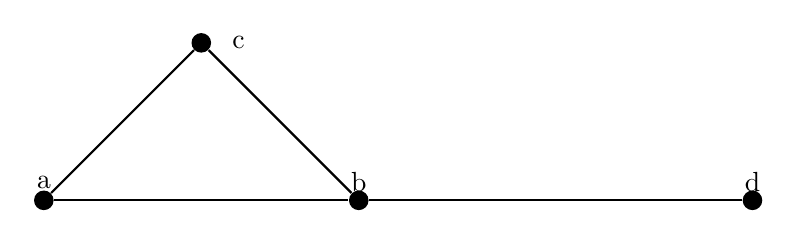
\begin{tikzpicture}[
  vertex/.style={circle, fill=black, inner sep=2.5pt}
]
  %% Vertices
  \node[vertex, label={[label distance=-3pt]above:{a}}] (a) at (0,0) {};
  \node[vertex, label={[label distance=-4pt]above:{b}}] (b) at (4,0) {};
  \node[vertex, label={[label distance=4pt]right:{c}}] (c) at (2,2) {};
  \node[vertex, label={[label distance=-4pt]above:{d}}] (d) at (9,0) {};

  %% Edges
  \draw[thick] (a) -- (b) -- (d);
  \draw[thick] (a) -- (c) -- (b);
\end{tikzpicture}

\medskip

\textbf{Example 3.} Here is formula involving the greek letters $\alpha, \beta$ and $\epsilon$:

\[
  \alpha^2 + \beta^2 = \epsilon^2.
\]

\end{document}
